\RequirePackage{etex}
\documentclass{beamer}
\usepackage[latin9]{inputenc}
\usepackage[ngerman]{babel}
\usepackage{amsmath}
\usepackage{listings}
\usepackage{color}
\usepackage{pictex}
\usepackage{tikz}
\usepackage{siunitx}

\title[CAN]{Controller Area Network}
\author{Dominik Eisele}
\institute[WSS]{Werner-Siemens-Schule}
\date{\today}
\subject{CAN}
\keywords{CAN, Controller Area Network}

\usetheme{Singapore}
\usecolortheme{rose}
\setbeamertemplate{navigation symbols}{}
\setbeamertemplate{footline}[frame number]
\beamersetuncovermixins{\opaqueness<1>{25}}{\opaqueness<2->{15}}

\definecolor{dkgreen}{rgb}{0,0.6,0}
\definecolor{gray}{rgb}{0.5,0.5,0.5}
\definecolor{mauve}{rgb}{0.58,0,0.82}

\lstset{language=C}
\lstset{numbers=left,
	numberstyle=\tiny,
	numbersep=5pt,
	breaklines=true,
	showstringspaces=false,
	frame=l ,
	xleftmargin=15pt,
	xrightmargin=15pt,
	basicstyle=\ttfamily\scriptsize,
	stepnumber=1,
	keywordstyle=\color{blue},		% keyword style
	commentstyle=\color{dkgreen},	% comment style
	stringstyle=\color{mauve}		% string literal style
}

%\AtBeginDocument{\addtobeamertemplate{block begin}{\setlength\abovedisplayskip{0pt}}}
%\AtBeginDocument{\addtobeamertemplate{block begin}{\setlength\abovedisplayshortskip{0pt}}}

\let\oldsqrt\sqrt 
\def\sqrt{\mathpalette\DHLhksqrt}
\def\DHLhksqrt#1#2{\setbox0=\hbox{$#1\oldsqrt{#2\,}$}\dimen0=\ht0
\advance\dimen0-0.3\ht0
%0.3 ist das Ma� f�r die Hakenl�nge, relativ zum Inhalt der Wurzel
\setbox2=\hbox{\vrule height\ht0 depth -\dimen0}%
{\box0\lower0.4pt\box2}}

\setcounter{tocdepth}{1}

\begin{document}

\begin{frame}
	\titlepage
\end{frame}

\begin{frame}{Inhalt}
	\tableofcontents
\end{frame}


\section{Allgemeine Informationen}
\subsection{Allgemeine Informationen-dots}

\begin{frame}{Geschichte} 
	\begin{itemize}
		\item 1983 von Bosch als serielles Feldbussystem entwickelt\\ \pause
		\item Ziel war die Reduzierung der Kabelbauml�nge in Fahrzeugen \\ \pause
		\item Zertifiziert nach  ISO 11898-2 und  ISO 11898-3 (High- und Low-Speed CAN) \\ \pause
		\item CAN besitzt eine sehr sichere Daten�bertragung, welche Echtzeitanforderungen gerecht wird 
	\end{itemize}
\end{frame}

\begin{frame}{Aufbau}
	\begin{figure}
		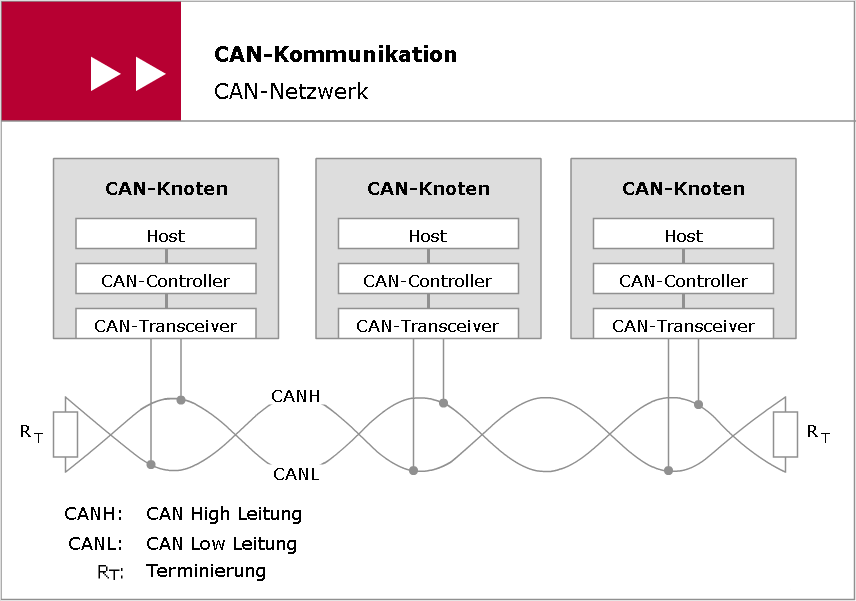
\includegraphics[width=\linewidth]{can_anschluss.PNG}
		\label{fig:aufbau}
	\end{figure}
\end{frame}


\begin{frame}{CAN-Buspegel}
	\begin{figure}
		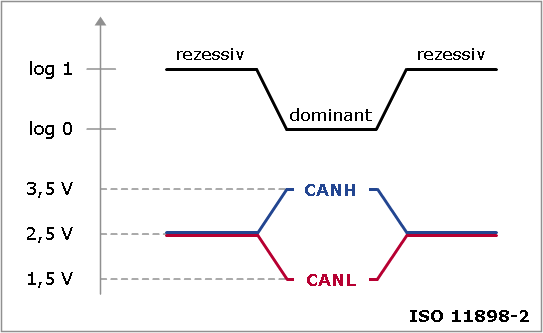
\includegraphics[scale=0.55]{can_highspeed.PNG}
		\label{fig:highspeed}
	\end{figure}
\end{frame}

\begin{frame}{CAN-Buspegel}
	\begin{figure}
		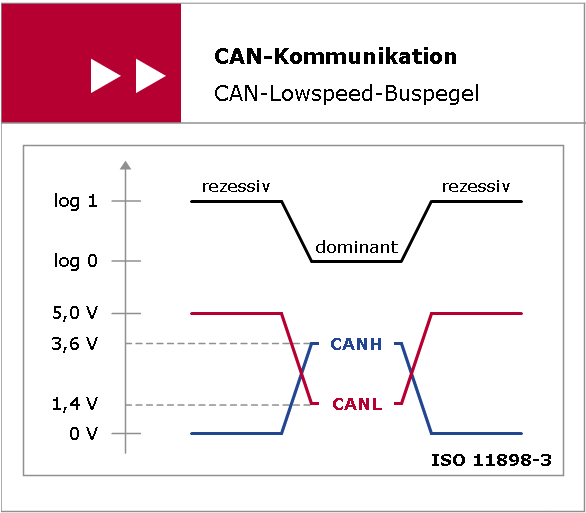
\includegraphics[scale=0.55]{can_lowspeed.PNG}
		\label{fig:lowspeed}
	\end{figure}
\end{frame}

\begin{frame}{Arbitrierung}
	\begin{itemize}
		\item CAN ist ein Multimasterbus, d.h. Teilnehmer m�ssen selbst entscheiden wann sie senden \\ \pause
		\item zum Einsatz kommt daher dass Carrier Sense Multiple Access/Collision Avoidance (CSMA/CA) Verfahren \\ \pause
		\item wenn zwei Teilnehmer gleichzeitig senden kommt die bitweise Arbitrierung zum Einsatz \\ \pause
		\item bei der Arbitierung werden die Identifier gleichzeitig gesendet und der Buspegel mit dem Sendepegel verglichen\\ \pause
		\item sendet ein Teilnehmer ein dominantes und ein anderer ein rezessives Bit wird der Buspegel dominant (logische 0)
	\end{itemize}
\end{frame}

\begin{frame}{Arbitrierung}
	\begin{figure}
		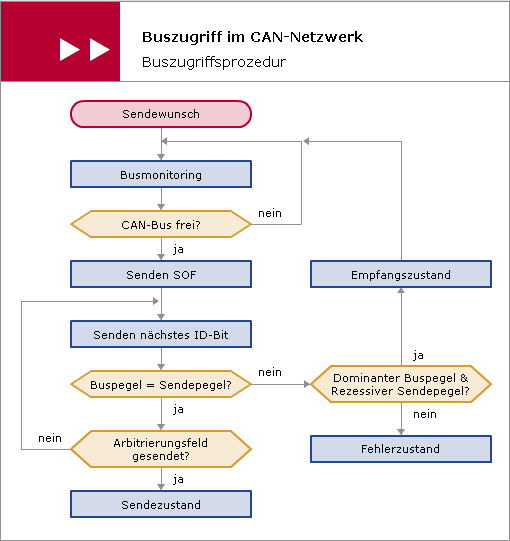
\includegraphics[scale=0.535]{buszugriff.PNG}
		\label{fig:buszugriff}
	\end{figure}
\end{frame}

\begin{frame}{Leitungsl�nge}
	\begin{figure}
		\begin{figure}[h!]
	\begin{tikzpicture}[xscale=0.8,yscale=0.6]
		% Achsen
		\draw[-] (0,0) -- (10,0) node[below] {\begin{tabular}{ll} \\  Leitungsl�nge in \si{\metre} \end{tabular}};
		\draw[-] (0,0) -- (0,9) node[below,left] {};
		\draw[-] (-1,4.5) -- (-1,4.5) node[left] {\begin{tabular}{l} k\\B\\i\\t\\s\\/\\s\end{tabular}};
		%Pfeile
		\draw[->] (0,0) -- (10,0);
		\draw[->] (0,0) -- (0,9);
		% Achsbeschriftung
		\foreach \x in {,1,...,9} \draw (\x,0.05) -- (\x,-0.05) node [below] {};
		\foreach \y in {1,...,8} \draw (0.1,\y) -- (-0.1,\y) node [left] {};		
		\draw (0,0) -- (0,0) node [below] {0};
		\draw (1,0) -- (1,0) node [below] {10};
		\draw (2,0) -- (2,0) node [below] {50};
		\draw (3,0) -- (3,0) node [below] {100};
		\draw (4,0) -- (4,0) node [below] {200};
		\draw (6,0) -- (6,0) node [below] {1000};
		\draw (9,0) -- (9,0) node [below] {10000};
		\draw (0,0) -- (0,0) node [left] {0};
		\draw (0,1) -- (0,1) node [left] {5};
		\draw (0,2) -- (0,2) node [left] {10};
		\draw (0,3) -- (0,3) node [left] {20};
		\draw (0,4) -- (0,4) node [left] {50};
		\draw (0,5) -- (0,5) node [left] {100};
		\draw (0,6) -- (0,6) node [left] {200};
		\draw (0,7) -- (0,7) node [left] {500};
		\draw (0,8) -- (0,8) node [left] {1000};
		\draw[smooth,samples=500,domain=0.0:8.24] plot(\x,{-0.062568 * \x^2 + -0.294511 * \x + 8.190863});
	\end{tikzpicture}
	\label{fig:Diagramm}
	\end{figure}
		\label{fig:leitunslaenge}
	\end{figure}
\end{frame}



\section{Protokoll}
\subsection{Protokoll-dots}
\begin{frame}{Aufbau }
dfsg
\end{frame}


\section{Anwendungen}
\subsection{Anwendungen-dots}
\begin{frame}{Aufbau }
dfsg
\end{frame}


\section{Quellen}
\subsection{Quellen-dots}
\begin{frame}{Quellen}
	\begin{itemize}
		\item Konrad Etschberger - CAN Controller-Area-Network Grundlegen, Protokolle, Bausteine, Anwedungen
		\item Praxis Profiline - Controller-Area-Network CAN in Automation (CiA)
		\item elearning.vector.com (30.06.2016)
	\end{itemize}
\end{frame}


\end{document}
